\scanpage{7}

% 1–7, realization of elements
Les éléments du $F_\alpha$ se réalisent comme parties \inserted{(à structure \unsure{cônique|conique|coniques})} de $|F_*|$ [\unsure{la ré.|la ré\textsuperscript{o}|associé} à $x\in F_{\unsure{n|\alpha}}$ correspond la réunion des simplexes réalisations des simpl. \deleted{fermés} \inserted{\unsure{corresp|ouverts}} d'élément $\leq x$], la relation d'incidence devient l'inclusion --- il y a une équivalence de catégories (\deleted{\unsure{top.}} d'objets top. versus objets combinatoires) à dégager.

% 8–10, proposition beside vertical rule
\uline{Prop} Si $|F_*|$ est une variété top. \inserted{\unsure{pure|petit|pointée}} de dim $n$, alors $(F_\alpha)$ satisfait les conditions $\deleted{\unsure{I}}1,1',2,2',3,4$\ldots

% 10–14, more precise criterion
[Plus précisément, pour que $(F_*)$ soit une variété top. de dim $n$, il f. et s. que $(F_*)$ satisfasse $1,1',2,2',3,3',4$, \uline{et} que $\forall x\in F_\alpha$, \inserted{$(\alpha\geq3)$}, la réalisation géom. de $F(x)$ soit une sphère

% 14–18, nested qualification
[en fait, \deleted{\unsure{et}} si on a l'hyp. de Poincaré, il suffit d'exiger que \deleted{pour $\alpha\geq\unsure{3,4|3?|3}$}, $|F(x)|$ soit simplement connexe et \deleted{ait} \inserted{pour $\alpha\geq5$, il ait de plus} l'homologie d'une sphère de m\textsuperscript{e} dimension.

% after 18, divider
\figure{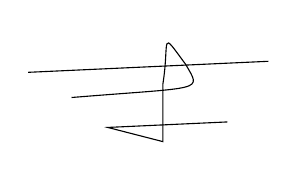
\begin{tikzpicture}[x=1cm,y=1cm]\draw (-1.55,.3)--(1.5,.44); \draw (-1,-.02).. controls (.7,.12) and (.65,.05) ..(.45,.4).. controls (.11,.86) and (.25,.72) ..(.16,.15)--(.16,-.58)--(-.54,-.4)--(.98,-.33);\end{tikzpicture}}

% 19–20, filtered space
Soit $X$ un espace top. \inserted{(\unsure{compact ?|compact ??})} filtré par
\[
 X_0\subset X_1\subset\ldots\subset X_n=X.
\]
\deleted{On suppose \unsure{$X$} est} \inserted{$X$ \unsure{var.} de dim $n$}

% 21–23, successive differences
que $\forall i=0,\ldots,n-1$, la \uline{différence} de $X_{i+1}$ suiv\textsuperscript{ant} $X_i$ est \deleted{une variété} \inserted{homéomorphe} à \deleted{boule de di\unsure{m}} \inserted{une} réunion de boules $D^{i+1}$.

% 23–26, flags of the filtration
Soit $\mathcal A$ l'ens des ``drapeaux'' relatifs à cette filtration (à définir avec soin). On a alors une op. de $G_{n\unsure{(+1)|+1}}$ (\deleted{\unsure{resp. =}} $G_n$ si $X$ \unsure{de la variété|déjà variété|variété} top. de dim $n$)

% lower left
% archive sheet number: 6
